\section{Literature survey methodology and results}
\label{section:2}

The first step of our survey was to obtain a list of candidate ontologies that could potentially include entities related to researcher information needs and its context.
%The purpose of this search is to find which domain parts have been addressed in which context and what has not been addressed yet. In this section, we describe our literature review process for finding relevant artifacts for further analysis.
%
Given the fact that most ontologies and relevant projects are %potentially 
%documented 
reported in %research articles 
papers, %and presented at  conference or published in a journal within the Semantic Web area, one of the best ways to find such articles is to search in online abstract and citation databases with bibliographic information on computer science publications. Portals that have high computer science article coverage include 
a major source to be searched were high-coverage bibliographic/citation databases, of which we considered \emph{Scopus},\footnote{\url{https://www.scopus.com/}}
\emph{Web of Science}\footnote{\url{https://webofknowledge.com}}
%, DBLP%\footnote{\url{https://dblp.org/}}
%, IEEE%\footnote{\url{https://ieeexplore.ieee.org/}}
%, and the ACM Digital Library%\footnote{\url{https://dl.acm.org/}}
%. The second tier of resourceful tools are search engines such 
and \emph{Google} Scholar.\footnote{\url{https://scholar.google.com/}}
%, Microsoft Academic%\footnote{\url{https://academic.microsoft.com/home}}
%, ScienceDirect%\footnote{\url{https://www.sciencedirect.com/}}
%, CORE%\footnote{\url{https://core.ac.uk/}} 
Additionally, we also directly asked the generic \emph{Google search engine}, to also cater for ontologies not accompanied with a paper for some reason.
The different resources are complemenary.
While the (top) Google/Scholar search should lead to popular resources with many inlinks/citations, the traditional bibliographic databases primarily return respectful academic publications (even those with lower citation response) and can be searched using more sophisticated means, thus reducing the amount of noice for the subsequent manual scan of results.
While there are, obviously, a number of other possible databases to consider (such as DBLP, or the IEEE/ACM libraries), we assumed that sufficient coverage can already be obtained via the four we chose.
Finally, for directly retrieving ontologies, an obvious choice was the \emph{Linked Open Vocabularies} (LOV) portal\footnote{\url{https://lov.linkeddata.es/}} 

%For obvious reasons, Google was our first bet. 
Using Google as the initial baseline,
%With this lax and quite naive approach 
we 
%managed to find a good amount of relevant ontologies using simple terms such as
searched for the most obvious phrases only, to keep the precision acceptable: \textit{scholar/ly ontology}, \textit{academic ontology}, \textit{research/er ontology}, and \textit{bibliography/ic ontology}.
%, \textit{conference ontology}
For each Google query, we examined the first 10 pages of results, 
%(approx. 160 results). sorted by relevance. Google results represented a list of mixed resources 
which consisted in a mix of publications, projects, and actual ontology documentations. %Nevertheless, over 80\% of the listed Google results were irrelevant or duplicated based on the result title. This approach apparently requires a lot of manual evaluation and is time-consuming but the results are acceptable. In this first iteration, 
Overall we identified, this way, a total of 9 relevant ontologies. 
%which, by their titles and description, indicate high relevancy.

%\begin{itemize}
%    \item Scholarly Ontology (SO)
%    \item Scholarly Event Description Ontology (SEDE)
%    \item FOAF-Academic Ontology
%    \item Researcher Profile Ontology for Academic Environment
%    \item Ontology for Academic Program Accredication (ABET)
%    \item Academic Institution Internal Structure Ontology (AIISO)
%    \item Curriculum, Course, and Syllabus Ontology (CCSO)
%    \item SPAR Ontologies
%    \item VIVO-ISF Ontology
    %\item Informatics Research Artifact Ontology
%\end{itemize}

We then used the Google Scholar search engine with the same search terms. 
%This time we expected a significant increase in the relevancy of the search results. 
Google Scholar returned, in all cases, publications, from which %such as articles and books. Search results were enhanced with bibliographic data such as authors, publication year, venue, citations, and related articles. Among the first ten pages of Google Scholar results (approx. 160 results), the relevancy was still very low topic-wise%, but almost all results were publications
%and there was still a lot of manual checking, reading the titles and abstracts. This time, 
we  collected 5 further relevant ontologies.

%\begin{itemize}
%    \item AcademIS Ontology
%    \item Computer Science Ontology (CSO)
%    \item BIBO Ontology
%    \item CiTO Ontology
%    \item Semantic Web for Research Communities Ontology (SWRC)
%\end{itemize}

Next, we used the Scopus bibliographic database.
%, launched in 2004. is a high-quality and easy-to-use database that covers an enormous amount of bibliographic records from a large number publishers including peer-reviewed journals. 
The advantage of searching in a specialized database was the higher degree of relevance 
%and completeness because the search is focused solely on scientific publications that have mandatory indicative data used for indexing. Another advantage in searching online is that it also, in some cases, provide the user with related articles with high relevancy and citation exports. This makes it much easier and faster to find projects that make use of the mentioned ontologies.  %Keyword-based search is better compared to general-purpose search on Google because the search terms is compared against multiple meta information of the publication such as title, keywords and abstract, which are indexed. %
To make a better use of the search tools provided by Scopus, we used our search terms to search for papers by titles and keywords, while limiting the scope to the Computer Science and Engineering fields. The following snippet represents our Scopus search query, which we used for searching in the title; analogous queries were applied on the abstract and keywords:
%\begin{Verbatim}[fontsize=\small]
%    TITLE ((academic OR scholarly OR researcher OR bibliography) 
%        AND  ontology) AND (SUBJAREA("COMP") OR  SUBJAREA("ENGI")) 
%\end{Verbatim}

\begin{lcverbatim}
TITLE ((academic OR scholarly OR researcher OR bibliography) 
    AND  ontology) AND (SUBJAREA("COMP") OR  SUBJAREA("ENGI")) 
\end{lcverbatim}

The search in the titles (TITLE) yielded 57 results, the search in abstracts (ABS) yielded 2829 results, and the search in keywords (KEY) yielded 279 results, all sorted by relevance. In the case of abstract-related results, we browsed the first 10 pages (approx. 100 results). Among these results, we found a total of 22 additional ontologies.
%The following list includes several more relevant ontologies for our research:

%\begin{itemize}
%    \item Ontology for Linked Open University Data (OLOUD)
%    \item Education Standards Ontology (ESO)
%    \item Education Application Ontology (EAO)
%    \item Funding, Research Administration and Projects Ontology (FRAPO)
%    \item PLET4Thesis
%    \item Open Research Knowledge Graph Ontology (ORKG)
%    \item Ontology for Academic Department
%    \item Academic Evaluation Ontology
%    \item Ontology for Academic Context Reasoning
%    \item FRBR-aligned Bibliographic Ontology (FaBIO)
%    \item Bibliographic Reference Ontology (BiRO)
%    \item Citation Counting and Context Characterisation Ontology (C4O)
%    \item Document Components Ontology (DoCO)
%    \item Publishing Status Ontology (PSO)
%    \item Publishing Roles Ontology (PRO)
%    \item Publishing Workflow Ontology (PWO)
%    \item Scholarly Contributions and Roles Ontology (SCoRO)
%    \item DataCite Ontology
%    \item Bibliometric Data Ontology (BiDO)
%    \item FAIR* Reviews Ontology (FR)
%    \item Five Stars of Online Research Articles Ontology
%    \item OpenCitations (OC)
%\end{itemize}

Our last bibliographic database of choice was the Web of Science.  First, we searched for each term one by one. The term \textit{scholarly ontology} yielded 32 results, the term \textit{academic ontology} yielded 87 results, the term \textit{researcher ontology} yielded 182 results (all with the refinement to the `article' document type and to the `computer science and information systems' category). Next, we used a query equivalent to the one used on Scopus, for searching in the title (and, analogously, in the topic) as follows:
%\begin{verbatim}
%    TI = ((academic OR scholarly OR researcher OR bibliography) 
%        AND ontology) AND SU = (Computer Science OR Engineering)
%\end{verbatim}
\begin{lcverbatim}
TI = ((academic OR scholarly OR researcher OR bibliography) 
    AND ontology) AND SU = (Computer Science OR Engineering)
\end{lcverbatim}
This query returned 22 results for the title filter (TI) and 423 results for the topic (TS) filter. Among these results, we found 2 additional ontologies.% were found.


%\begin{itemize}
%    \item UniGrad (FOAF+SIOC extension)
%    \item Extension of the BiDO Ontology to Represent Scientific Production (BSBM)
%\end{itemize}

% http://www.scholarlydata.org/sparql/


%After a couple of search , we quickly realized that, in most cases, the resulting publications were overlapping and the number of new results was decreasing. The number of collected results each time depends on the order of chosen tools and thus does not reflect the true resourcefulness of the databases. %For that reason we did not search further on IEEE, ACM DL, Microsoft Academic, Science Direct and CORE.

Aside the keyword-based search, we also benefited from the availability of \emph{citation links} in Google Scholar, Scopus and Web of Science. 
We followed some promising incoming citation links to the papers on ontologies found so far. 
%for more papers involving ontologies that we missed during the keyword-based search. 
Using this technique, we identified 3 further ontologies.

For each ontology found through a paper reporting on it, we as much information as possible, including its metadata, source code and full texts of the referencing papers (when available). 

%\begin{itemize}
%    \item SemSur: Core Ontology for the Semantic Representation of Research Findings
%    \item Ontology for describing academic mental states
%    \item KISTI Reference \& Academic Ontology
%\end{itemize}


%Although our scope of focus is not too large, the search results could still be overwhelming in number which need proper filtering and narrowing down. 

% On the other hand, the keyword-based search might not be complete due to synonymy etc. 

Last, 
%because there is a good chance these 
we directly searched for ontologies  %listed 
on the LOV portal. We %did a thorough search on this portal and 
found a considerable amount of relevant resources using the keywords \textit{research}, \textit{academic}, \textit{scholar} and \textit{bibliography}, of which most had already been
covered by the previous bibliographic database or Google results.  
However, two new relevant ontologies were still found this way. % probably because of too generic naming:

We then used the LOV results as a referencing resource to find related literature that described them (and  possibly escaped the previous literature search), projects that used them,
%\begin{itemize}
%    \item Research Object Ontology (RO)
%    \item Common European Research Information Format Ontology (CERIF)
%\end{itemize}
as well as to complete the missing information such as the namespaces and links to the source code. 

%To reduce future problems related to both imprecision and incompleteness of a naive keyword search
To facilitate running a similar process in the future, we briefly summarize our literature search protocol for finding state-of-the-art ontology data:

\begin{enumerate}
    \item determine search engines and relevant online databases, %(based on search samples from multiple portals, results were often overlapping, so we recommend to use only Scopus which has the best tools for filtering),
    \item define search criteria for optional filtering which include the top-level field, topic or domain, and keywords including their combinations,
    \item execute initial search and iterate through an adequate amount of results,
    \item exclude duplicate articles among the initial results,
    \item manually include relevant articles based on title, keywords and abstract,
    %\item exclude articles that introduce work that are in early phase of development such as poster papers, PhD papers
    %\item exclude articles that do not mainly introduce an ontology or its usage in an applied project, [provide at least 2 examples which where excluded]
    \item since search by keyword can miss some papers, try reverse citation tracking, even if paper is weak (has not been cited many times), forward tracing, reverse tracking of citations, since a later work could include a comparison of such papers,
    \item look for ontologies in online specialized catalogs such as LOV.
\end{enumerate}

In Figure \ref{literature-review}, we provide an overview of this literature survey procedure.
\begin{figure}
\centering
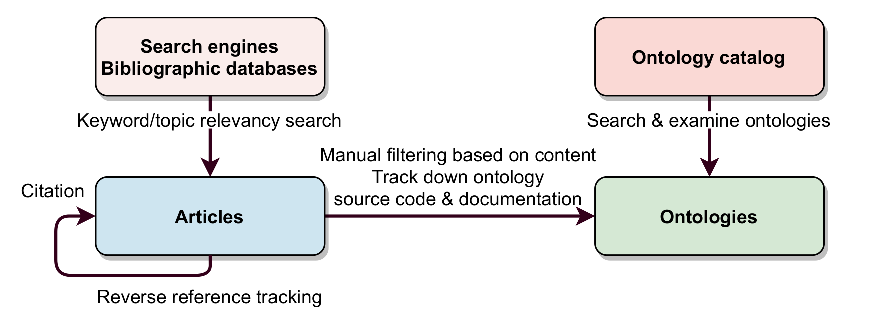
\includegraphics[width=9cm]{figures/literature-review.eps}
\caption{
    %Conceptual model for exploring literature, 
    Procedure for retrieving ontology related resources.} \label{literature-review}
\end{figure}

%The following is the list of keywords used in both literature search and LOV.
%\begin{itemize}
%    \item scholar/ly ontology,
%    \item academy/ic ontology,
%    \item research/er ontology,
    % \item publishing ontology,
    % \item referencing ontology, 
    % \item ontology for describing bibliographic resources and citations, 
    % \item ontology for describing bibliography, 
    %\item citations ontology, 
%    \item bibliography/ic ontology, 
%\end{itemize}

The result of our survey was a comprehensive table of metadata related to the ontologies. 
However, there were still some incomplete records due to unavailable or missing information.
%The next step is to examine the discovered ontologies at the 
Content-level analysis also revealed some ontologies that were likely irrelevant for practical information search, e.g., an `Ontology for describing academic mental state'. 
From the totality of 43 ontologies found, we thus eventually chose 34 for which 1) we deemed the availability of source code and/or metadata sufficient for effective reuse, and 2) the ontology content was indeed relevant to researcher information needs.
Table \ref{tab:research-related-ontologies}
%and \ref{tab:research-bib-related-ontologies} 
shows the final list of ontologies\footnote{Some acronyms in this table are unofficial, e.g. OAD or RPO, and are only introduced for convenient referencing within this research.} used in our subsequent analysis.

\begin{table}[]
\centering
\caption{Research-related ontologies}
\label{tab:research-related-ontologies}
\begin{tabular}{llr}
\toprule
\textbf{Acronym} & \textbf{Name}                                                                             \\ \midrule
SO            & Scholarly Ontology & \cite{DBLP:journals/jodl/PertsasC17}                                      \\ \midrule
OLOUD         & Ontology for Linked Open University Data & \cite{10.12700/APH.14.4.2017.4.4}                   \\ \midrule
VIVO          & VIVO-ISF Ontology & \cite{DBLP:series/synthesis/2012Borner}                                    \\ \midrule
CCSO          & Curriculum, Course, and Syllabus Ontology & \cite{DBLP:conf/esws/KatisKAV18}                   \\ \midrule
AIISO         & Academic Institution Internal Structure Ontology & \cite{DBLP:conf/incos/KalemiM11}            \\ \midrule
FRAPO         & Funding, Research Administration and Projects Ontology & \cite{Frapo}                          \\ \midrule
ORKG          & Open Research Knowledge Graph & \cite{DBLP:conf/kcap/OelenJFSA19}                              \\ \midrule
ESO \& EAO    & Education Standards \& Education Application Ontology & \cite{DBLP:conf/semweb/RashidM18}      \\ \midrule
SEDE          & Ontology for Scholarly Event Description & \cite{DBLP:journals/jis/JeongK10}                   \\ \midrule
OAD           & Ontology for Academic Department & \cite{An:OAD}                                               \\ \midrule
AcademIS      & AcademIS Ontology & \cite{DBLP:conf/pci/TriperinaST13}                                         \\ \midrule
CSO           & The Computer Sciene Ontology & \cite{DBLP:conf/semweb/SalatinoTMOM18}                          \\ \midrule
BIBO          & The Bibliographic Ontology & \cite{bibo}                                                       \\ \midrule
FOAF-Academic & FOAF-Academic Ontology & \cite{DBLP:conf/incos/KalemiM11}                                      \\ \midrule
%PLET4Thesis   & PLET4Thesis & \cite{DBLP:conf/icetc/Tapia-LeonSCL17}                                           \\ \midrule
SemSur        & Semantic Survey Ontology & \cite{DBLP:conf/i-semantics/FathallaVA018}                          \\ \midrule
RO            & Research Object Ontology & \cite{DBLP:journals/corr/BelhajjameZGHPCGBKG14}                     \\ \midrule
SWRC          & Semantic Web for Research Communities & \cite{DBLP:conf/epia/SureBHHO05}                       \\ \midrule
ABET          & Ontology for Academic Program Accreditation & \cite{10.14569/IJACSA.2016.070717}               \\ \midrule
RPO           & Researcher Profile Ontology for the Academic Environment & \cite{DBLP:conf/cvc/BravoRC19}      \\ \midrule
%IRAO          & Informatics Research Artifacts Ontology                                                     \\ \midrule
CERIF         & Common European Research Information Format Ontology & \cite{DBLP:journals/datascience/Jorg10} \\ \midrule
FaBiO         & FRBR-aligned Bibliographic Ontology & \cite{DBLP:journals/ws/PeroniS12}                        \\ \midrule
CiTO          & Citation Typing Ontology & \cite{DBLP:journals/ws/PeroniS12}                                   \\ \midrule
BiRO          & Bibliographic Reference Ontology & \cite{DBLP:conf/esws/IorioNPSV14}                           \\ \midrule
C4O           & Citation Counting and Context Characterisation Ontology & \cite{DBLP:conf/semweb/OsbornePM14}  \\ \midrule
DoCO          & Document Components Ontology & \cite{DBLP:journals/semweb/ConstantinPPSV16}                    \\ \midrule
PSO           & Publishing Status Ontology & \cite{DBLP:conf/i-semantics/PeroniSV12}                           \\ \midrule

%\\ \bottomrule

%\end{tabular}
%\end{table}

%\begin{table}[]
%\caption{Research-related ontologies}
%\label{tab:research-bib-related-ontologies}
%\begin{tabular}{ll}
%\toprule
%\textbf{Acronym} & \textbf{Name}   \\ \midrule
PRO           & Publishing Roles Ontology & \cite{DBLP:conf/i-semantics/PeroniSV12}                            \\ \midrule
PWO           & Publishing Workflow Ontology & \cite{DBLP:journals/semweb/GangemiPSV17}                        \\ \midrule
SCoRO         & Scholarly Contributions and Roles Ontology & \cite{Scoro}                                      \\ \midrule
DataCite      & DataCite Ontology & \cite{DataCite_Ontology}                                                   \\ \midrule
BiDO          & Bibliometric Data Ontology & \cite{tapia2019extension}                                         \\ \midrule
FiveStars     & Five Stars of Online Research Articles Ontology & \cite{DBLP:journals/dlib/Shotton12}          \\ \midrule
FR            & FAIR* Reviews Ontology & \cite{Fair}                                                           \\ \midrule
%BSBM          & Extension of the BiDO Ontology to Represent Scientific Production & \cite{tapia2019extension}  \\ \midrule
OCO           & OpenCitations Ontology & \cite{DBLP:journals/qss/PeroniS20}

\\ \bottomrule

\end{tabular}
\end{table}



% 

\medskip
\noindent \textbf{Description of ontologies}

\medskip
\noindent \textbf{OLOUD-BASE} \& \textbf{OLOUD-LOC}. \cite{10.12700/APH.14.4.2017.4.4} The objectives of the OLOUD ontology is to support the development and publishing of Linked Open University Datasets and the applications built on the top of these Open Datasets. OLOUD contains classes and properties to describe Organizations, People, their Roles and Publications, Subjects, Courses and other Events and their temporal and spatial description. The ontology is divided into two connected modules: 1. OLOUD-BASE is the main module describing all the university related concepts and uses the prefix \texttt{oloud}, 2. OLOUD-LOC module provides the indoor location and navigation features and uses the prefix \texttt{loc}.

\medskip
\noindent \textbf{VIVO}. \cite{DBLP:series/synthesis/2012Borner} An ontology of academic and research domain, developed in the framework of the VIVO project. It represents researchers in the context of their experience, outputs, interests, accomplishments, and associated institutions.

\medskip
\noindent \textbf{SWRC}. \cite{DBLP:conf/epia/SureBHHO05} An ontology for modeling entities of research communities such as persons, organisations, publications (bibliographic metadata) and their relationship.

\medskip
\noindent \textbf{ABET}. \cite{10.14569/IJACSA.2016.070717} Ontology of Accreditation Board of Engineering and Technology Process. It helps faculty  or  curriculum  committees  avoid  over  mapping  or  under mapping students' outcomes.

\medskip
\noindent \textbf{CCSO}. \cite{DBLP:conf/esws/KatisKAV18} This Ontology aims to provide data model for describing the subjects of Curriculum, Course and Syllabus in Higher education. Using this ontology, syllabus items can be effectively described and annotated enabling intelligent systems to support teaching and learning by offering automated services like syllabus semantic searching, matching and interlinking, syllabus recommendation and evolution.

\medskip
\noindent \textbf{FOAF-Academic}. \cite{DBLP:conf/incos/KalemiM11} A Vocabulary for the Academic Community. This ontology helps the academic community in saying anything about their achievements, their qualifications, activities and the communities that are near to them.

\medskip
\noindent \textbf{AIISO}. \cite{DBLP:conf/incos/KalemiM11} The Academic Institution Internal Structure Ontology (AIISO) provides classes and properties to describe the internal organizational structure of an academic institution.

\medskip
\noindent \textbf{ESO} \& \textbf{EAO}. \cite{DBLP:conf/semweb/RashidM18} Education Application Ontology and Education Application Ontology are used to simplify lesson planning for teachers, providing support for students by linking relevant resources, and providing a potential terminology for use in a lingua-franca for communicating with multiple communities about education components.

\medskip
\noindent \textbf{PLET4Thesis}. \cite{DBLP:conf/icetc/Tapia-LeonSCL17} The PLET4Thesis ontology is designed in order to organise the process of thesis development using the elements required to create a PLE (personal leaning environment).  Designed to guide thesis students in the construction of their PLE.

\medskip
\noindent \textbf{ORKG}. \cite{DBLP:conf/kcap/OelenJFSA19} The Open Research Knowledge Graph Ontology is used for comparing research contributions in a scholarly knowledge graph.

\medskip
\noindent \textbf{Researcher Profile Ontology}. \cite{DBLP:conf/cvc/BravoRC19} This ontology is designed specifically to represent academic contexts at a public university. It supports the representation of researcher profiles in a given academic environment.

\medskip
\noindent \textbf{IRAO}. Used to describe research artifacts in research, including authorship, evolution, etc.

\medskip
\noindent \textbf{CERIF}. \cite{DBLP:journals/procedia/JorgLK12} The Common European Research Information Format (CERIF) Ontology Specification provides basic concepts and properties for describing research information as semantic data. This document contains a friendly description of the Common European Research Information Format (CERIF) Ontology developed by EuroCRIS.

\medskip
\noindent \textbf{RO}. \cite{DBLP:journals/ws/Belhajjame0GGHP15} The Research Object Ontology provides basic structure for the description of aggregated resources and the annotations that are made on those resources.




%add by gollam rabby
% start

\medskip
\noindent \textbf{FaBiO}. FaBiO\cite{DBLP:journals/ws/PeroniS12} is an ontology applied for describing the entities that are published or undeniably publishable works (e.g. journal articles, conference papers, books), that contain or suggest bibliographic references. It also covers data sets, web pages, blogs, computer algorithms, formal specifications and vocabularies, experimental protocols, legal records, technical and commercial reports, governmental papers and similar publications, and also anthologies, catalogs, and corresponding collections. FaBiO has been developed to overcome any restriction to the classes and the domains with ranges of its properties. It is flexible and it has a superb advantage of allowing itself to be used side by side with other models.

\medskip
\noindent \textbf{CiTO}. CiTO\cite{DBLP:journals/biomedsem/Shotton10} is an ontology that allows characterization of the character or type of citations, both factually and rhetorically. Properties and consequently their inverses could even be classified as rhetorical and/or factual, with the rhetorical properties being grouped in three sets: positive, informative (neutral), or negative. The domain and range constraints from this thing and also properties aren't defined, so this ontology is easily integrable with other ontology models, like FaBiO. Two other ontologies are defined explicitly for describing specific aspects of CiTO, the first one is called Functions of Citations Ontology (FOCO) and the other one is called CiTO to Wordnet Ontology (C2W).

\medskip
\noindent \textbf{BiRO}. BiRO\cite{DBLP:conf/esws/IorioNPSV14} is an ontology designed to define the bibliographic records, bibliographic references, and their compilation into bibliographic collections and lists. This ontology also uses an OWL-based definition of the FRBR model\cite{bowen2011frbr} to identify the bibliographic references and their compilation into ordered bibliographic lists.

\medskip
\noindent \textbf{C4O}. C4O\cite{DBLP:conf/semweb/OsbornePM14} also provides the ontological structures which permit to record the amount of in-text citations, alongside their textual citation contexts and also the number of citations a cited entity has received globally on a specific date. It is also useful to explain how references are utilized in the citing paper. 

\medskip
\noindent \textbf{DoCO}. DoCO\cite{DBLP:journals/semweb/ConstantinPPSV16} is an ontology that organizes structured vocabulary from written document components following both structural (e.g. block, inline, paragraph, section, chapter) and rhetorical (e.g. introduction, discussion, acknowledgments, reference list, figure, appendix) options. It also imports the Pattern Ontology which describes the structural patterns, and therefore the Discourse Element Ontology (DEO), which was developed with DoCO to explain the rhetorical components. DoCO also defines hybrid classes to describe elements that are both structural and rhetorical in nature, like paragraph, section, or list. In addition, it aligned with the SALT Rhetorical Ontology and therefore the Ontology of Rhetorical Blocks (ORB).


\medskip
\noindent \textbf{PSO}. PSO\cite{DBLP:conf/i-semantics/PeroniSV12} ontology is designed and developed according to the TVC pattern, to characterize the publication status (e.g. draft, submitted, under review, etc.) of documents at every stage of the publishing process. Documents hold a specific status at a specific time as an immediate consequence of a particular event. Other pre-existing ontologies describing the status of documents (e.g. BIBO), rely on the specific property links but PSO prevents a correct description of scenarios.  

\medskip
\noindent \textbf{PRO}. PRO\cite{DBLP:conf/i-semantics/PeroniSV12} is an ontology that also uses the TVC pattern for characterization of the roles of agents (e.g. people, corporate bodies, and computational agents) within the publication process. Most of the time, the agents are authors, editors, reviewers, publishers, or librarians. It defines publishing roles as crucial as providing an entire description of a scholarly resource like a paper or a dataset.  

\medskip
\noindent \textbf{PWO}. PWO\cite{DBLP:journals/semweb/GangemiPSV17} is an ontology with two main classes called Workflow and Step, used for describing the steps of the workflow related to the publication of a document or other publication entity.

\medskip
\noindent \textbf{SCoRO}.SCoRO\cite{Scoro} is the Scholarly Contributions and Roles Ontology (CERIF-compliant ontology) for describing the contributions of authors, publishers, students, and research administrators. It is possibly used in those organizations where they're members with concerning projects, research investigations, and other academic activities focusing on scholarly journal articles and other outputs.

\medskip
\noindent \textbf{FRAPO} FRAPO\cite{Frapo} is the Funding Research Administration and Projects Ontology, which also uses a CERIF-compliant ontology for describing administrative information concerning grant funding and research projects. It also imports FOAF for characterizing people. It is mostly used for the characterization of grant applications, funding bodies, research projects, project partners, etc (the type of data stored in Current Research Information Systems (CRIS)). It also can be described as other sorts of projects, for instance, building projects and academic projects.

\medskip
\noindent \textbf{DataCite}. The main intent of the DataCite\cite{DataCite_Ontology} Ontology is to stock a versatile mechanism to prescribe the identifier for bibliographic resources and related entities. it also allows supplying a link between a resource and therefore the document describing its metadata utilizing CiTO, using the property citesAsMetadataDocument, and FaBiO, through the category of MetadataDocument. Additionally, to those entities, the DataCite Ontology provides appropriate classes and properties to specify the actual scheme followed to create the resource metadata exemplified within the metadata document.


\medskip
\noindent \textbf{BiDO}. BiDO\cite{tapia2019extension} developed a well-known model for enabling the classification of authors and journals consistent with bibliometric data, also share and reuse the data during a different context. The core module of the ontology allows one to explain any entity and therefore the related bibliometric data at a particular time and consistent with a particular agent. BiDO consists of three different modules and people are Standard bibliometric measures, Research career categories, and Review measures.

\medskip
\noindent \textbf{FiveStars}. To measure the standard of any multidimensional online journal a five stars' constellation like approach is followed by Five Stars of Online Journal Articles. The properties which are considered as stars are review quality, accessibility, content enrichment, availability of datasets and the machine-readable metadata. Articles of the online journals are evaluated based on these properties to enhance research quality and communications. This five star based conceptual framework is undoubtedly very helpful for researchers and other personnel's associated with journal publishing.\cite{DBLP:journals/dlib/Shotton12}

\medskip
\noindent \textbf{FAIR}.  FAIR \cite{Fair} is a review ontology (FR) that identifies a group of classes, properties, and axioms for describing research reviews as semantic objects and also reuse standard existing vocabularies by utilizing ontology engineering techniques.


\medskip
\noindent \textbf{BSBM}. BSBM\cite{tapia2019extension} is an enhancement of the BiDO Ontology, particularly BiDO Standard Bibliometric Measures.


\medskip
\noindent \textbf{OC}. The OpenCitations Data Model (OCDM)\cite{DBLP:journals/corr/abs-1906-11964} is the metadata model used for the stored information all together in the OpenCitation datasets. OCDM also allows us to record information about published bibliographic resources,https://www.overleaf.com/project/5ebbc2be39c6e30001174487 possible resource embodiments, bibliographic references, responsible agents, roles, citations, and external identifiers.


\medskip

 %end